\documentclass[../report.tex]{subfiles}
\begin{document}	

\chapter{Design and simulation}
\gls{tpr} can be achieved in different ways, discussed in section \ref*{sec:active_pr}. In this thesis, the goal is to achieve \gls{tpr} using MEMS for a broadband transmission, including the C and L bands. Moreover, the idea is to optimize the design to achieve high \gls{per} and low \gls{il}.  
	
	\section{Approach}
	\gls{mems} \gls{tpr} design can be approached in 2 ways. In a first approach, initially a passive \gls{pr} can be designed by introducing asymmetry and a MEMS tunable waveguide is introduced which impedes polarization rotation by reintroducing symmetry in the effective waveguide. In a second approach, the technique is reversed i.e. the MEMS tunable waveguide is used to introduce asymmetry in the waveguide structure which rotates polarization. Without the MEMS structure the polarization is not rotated. In the design principle of the \gls{tpr} described here, the first approach is being followed.  
	
	\section{Designing TPR}
	To design the geometry of the waveguide, standard mode solver software is used. Both, Comsol\cite{comsol_2015} and CST \cite{cst_2015} are used to solve the modes in equation \ref{eq:helmholtz_eq_wg_general}. Mostly, in this thesis, Comsol is used to find and optimize the modes in waveguide cross-section in 2-D geometry. Whereas, CST is used to optimize the 3-D structure by studying the transmission parameters of the wave (S-parameters).
	
	% obtained for output port mode after running the simulation. Air cladding is considered around the Silicon base waveguide for setting up the simulation.
		
		\subsection{Design principle}
To design a \gls{pr} in nanometer scale, precision is a key factor. Meshing of the geometry, cladding dimensions and its material composition, frequency range of the solvers, boundary conditions, volume of simulated area chosen, etc. are the key things to watch for in designing the simulation in the mode solver softwares. Also, the waveguides are suspended to accommodate the movement of the \gls{mems} tunable waveguide, which in turns changes the effective \gls{ri} of the mode. Hence, air cladding is used in the mode simulations in the waveguide cross-section. Moreover, as the idea is to make the \gls{tpr} as broadband as possible, it is necessary to do frequency analysis simulation for a wide-band spectrum in which the optical fibers for telecommunications work. As the operating wavelength of the telecommunications optical fiber network in C-band and L-band are between $\SI{1530}{\nano\metre}$ and $\SI{1625}{\nano\metre}$, the corresponding frequency range becomes $\SI{195.94}{\THz}$ - $\SI{184.48}{\THz}$.
	
		\subsection{Design: Mode hybridization based single stair Si waveguide with air cladding}

If, a light source polarized at an angle $\chem{\theta}$, is incident on a half wave plate (\ref{concept:wave_plates}), then the final \gls{sop} is derived using Jones matrix (\ref{concept:jones_matrix}), described as follows:

\begin{equation}\label{eq:wave_plate_pr}
\left( \begin{matrix} 1& & 0\\ 0& & -1\end{matrix} \right) \left( \begin{matrix} \cos \theta \\ \sin \theta \end{matrix} \right) ~ = ~ \left( \begin{matrix} -\cos \theta \\ -\sin \theta \end{matrix}\right) ~ = ~ \left( \begin{matrix} \cos \left(-\theta\right) \\ \sin \left(-\theta\right) \end{matrix} \right), 
\end{equation}
where, $\chem{\left( \begin{matrix} 1& & 0\\ 0& & -1\end{matrix} \right)}$ is the Jones matrix for the half wave plate derived using \ref{eq:jones_matrix_wp3} and $\chem{\left( \begin{matrix} \cos \theta \\ \sin \theta \end{matrix} \right)}$ is the Jones vector representation of linearly polarized wave at an angle $\chem{\theta}$, with the horizontal, derived using \ref{eq:jones_vector_general_form}. This concludes that an incidence of $\chem{\theta}$, produces an output of $\chem{-\theta}$, when passed through a wave plate, which gives $\chem{2\theta}$ polarization rotation. Thus to rotate polarization by $\chem{90{^\circ}}$, an incidence of $\chem{45{^\circ}}$ is necessary on the wave plate. The single stair waveguide acts as an wave plate due to its asymmetric structure which guides hybrid modes. To find out the dimensions for obtaining $45{^\circ}$ hybridized modes in the single stair waveguide, Comsol 2D mode solver software is used. 

\subsubsection{Waveguide geometry}
Throughout the next sections the dimensions of the stair waveguide are defined in terms of rib, slab and base described in Fig. \ref{fig:4_wg_structure}.   

\begin{figure}[H] %h
	\centering
	\includegraphics[width=0.43\textwidth]{4-wg-structure}
	\caption{Stair waveguide geometry}
	\label{fig:4_wg_structure}
\end{figure}


\subsubsection{Optimized dimensions of primary PR waveguide}
The dimensions of the stair waveguide is optimized to get hybridized modes. At $45{^\circ}$, the components of the E-fields in the hybridized modes must be such that, $E_X \approx E_Y$. It is necessary to double check the E-fields orientation to make sure that only the correct modes are chosen because in simulation a larger cross-section than the waveguide cross-section is excited. This excitation might produces modes for which $E_X \approx E_Y$, but the modes are not hybridized at $45{^\circ}$. Hence, for modes hybridized at $45{^\circ}$, $\dfrac {Avg(E_{X_{mode}})} {Avg(E_{Y_{mode}})} \rightarrow 1$. As a result, 

\begin{equation}\label{eq:wg_dim_eq}
\mathrm{Electric ~ field ~ ratio ~ in ~ hybrid ~ modes} ~ = ~ \sum _{mode}\mathrm{Real}\left| \log _{10}\dfrac {Avg(E_{X_{mode}})} {Avg(E_{Y_{mode}})}\right| \rightarrow 0. 
\end{equation}

\begin{figure}[H] %h
	\centering
	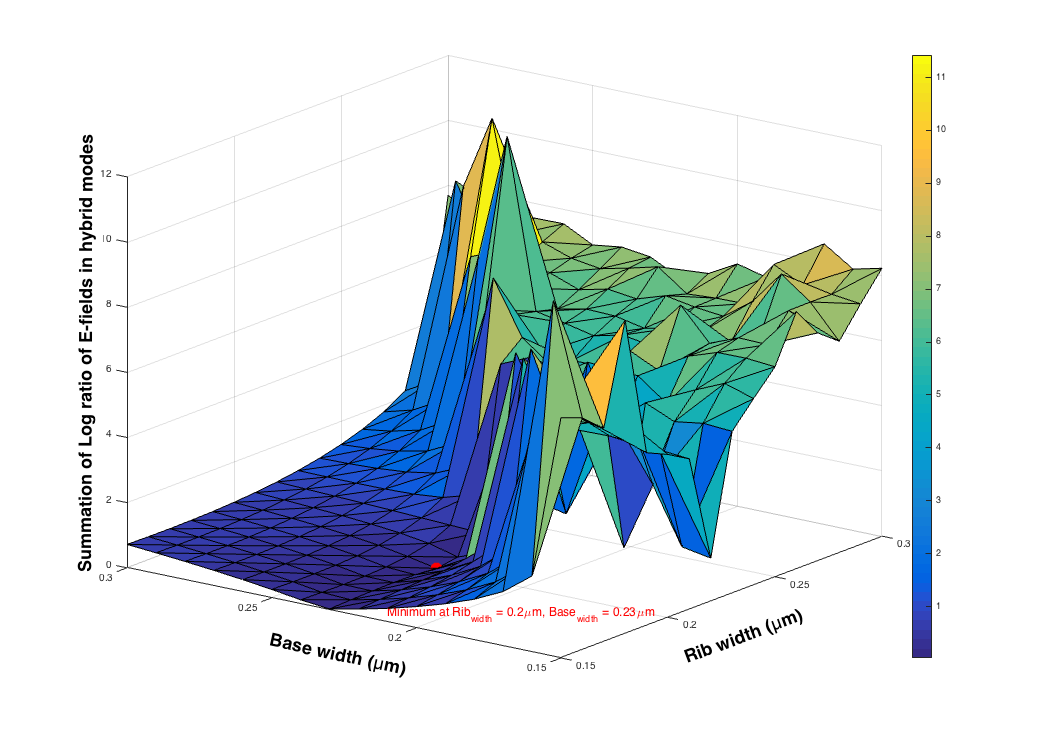
\includegraphics[width=1\textwidth]{4-graph-mode-sum}
	\caption{Summation of real part of absolute value of the logarithmic ratio of $E_x$ and $E_y$ fields plotted against rib and base width in an area chart using MATLAB}
	\label{fig:4_graph_mode_sum}
\end{figure}  
\noindent Hence, the minimum point on the graph represents the best dimensions on the waveguide for obtaining the hybridized modes at $45{^\circ}$. In this case the best dimensions were obtained at $\chem{Base_{width}}$ = \SI{230}{\nano \meter} and $\chem{Rib_{width}}$ = \SI{200}{\nano \meter}. The total height of the waveguide is \SI{220}{\nano \meter} because of the wafers available in lab. The $\chem{Slab_{height}}$ = \SI{110}{\nano \meter}, since the gratings are deigned and optimized for \SI{110}{\nano \meter}. Hence, a change in slab height or a double stair waveguide would increase the fabrication steps. It can also be visualized that, in the modes in Fig. \ref{fig:4_mode1_200_230} and Fig. \ref{fig:4_mode2_200_230}, that the effective modes are hybridized at $45{^\circ}$ for the first 2 hybrid modes obtained using Comsol simulation. 

\begin{figure}[H] %h
	\begin{subfigure}[t]{0.45\textwidth}
		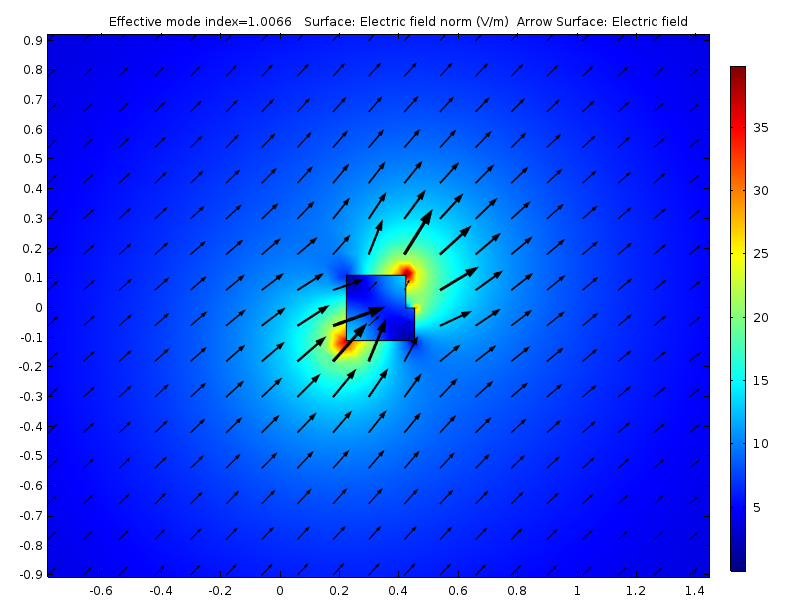
\includegraphics[width=\textwidth]{4-mode1-200-230}
		\caption{$1^{st}$ hybrid mode in the cross-section}
		\label{fig:4_mode1_200_230}
	\end{subfigure}
	\hfill
	\begin{subfigure}[t]{0.45\textwidth}
		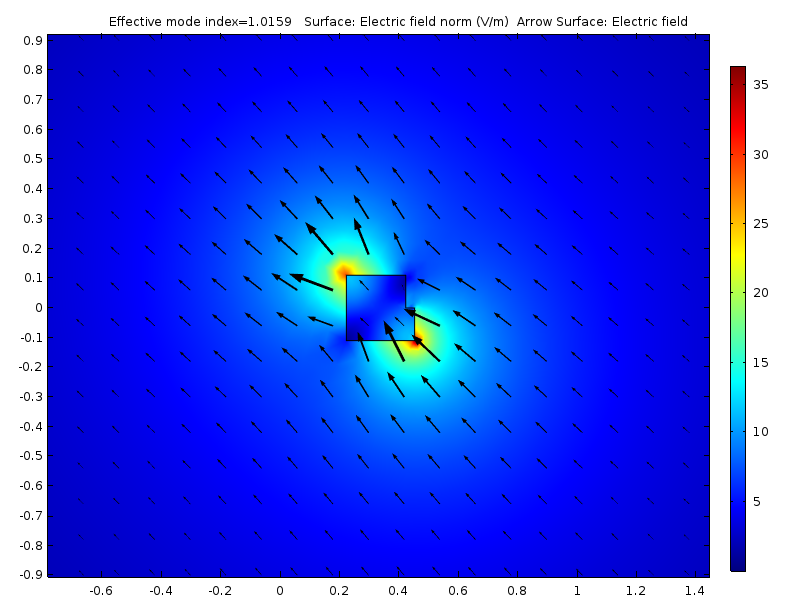
\includegraphics[width=\textwidth]{4-mode2-200-230}
		\caption{$2^{nd}$ hybrid mode in the cross-section}
		\label{fig:4_mode2_200_230}
	\end{subfigure}
	\caption{Fundamental hybrid modes in the cross-section with $\chem{Rib_{width}}$ = \SI{200}{\nano \meter}, $\chem{Rib_{height}}$ = 110nm, $\chem{Base_{width}}$ = \SI{230}{\nano \meter}, $\chem{Slab_{height}}$ = \SI{110}{\nano \meter}, obtained using Comsol 2-D eigenmode simulation}
\end{figure}

\begin{figure}[H] %h
	\begin{subfigure}[t]{0.45\textwidth}
		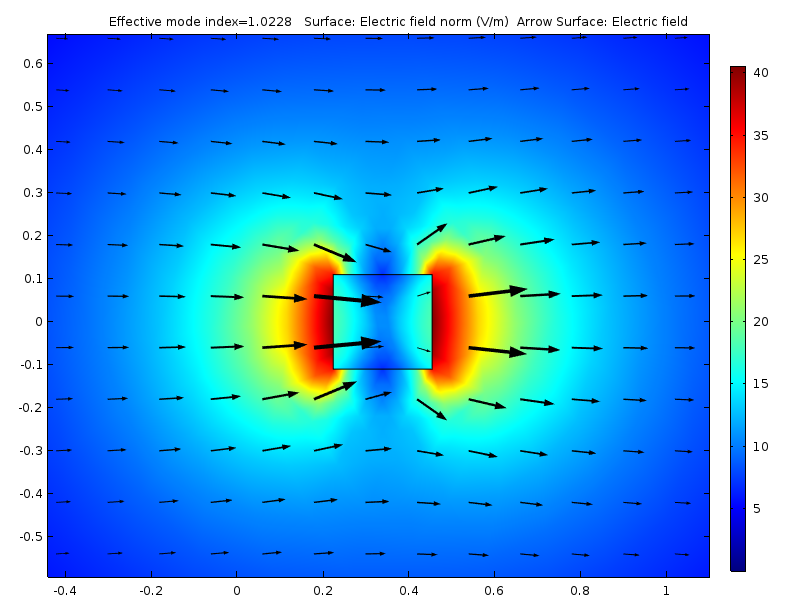
\includegraphics[width=\textwidth]{4-mode1-230-230}
		\caption{\gls{te} mode in the cross-section}
		\label{fig:4_mode1_230_230}
	\end{subfigure}
	\hfill
	\begin{subfigure}[t]{0.45\textwidth}
		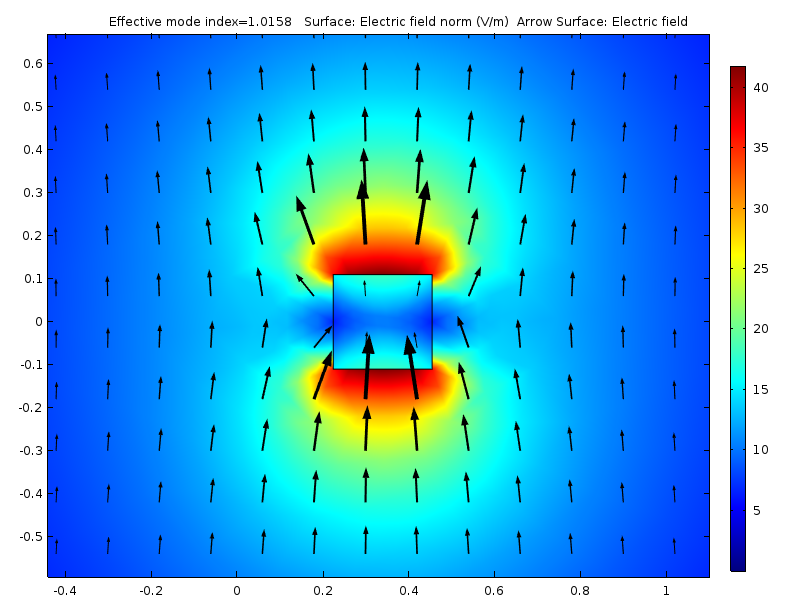
\includegraphics[width=\textwidth]{4-mode2-230-230}
		\caption{\gls{tm} mode in the cross-section}
		\label{fig:4_mode2_230_230}
	\end{subfigure}
	\caption{Fundamental modes in the cross-section with Width = \SI{230}{\nano \meter}, Height = \SI{220}{\nano \meter}, obtained using Comsol 2-D eigenmode simulation}
\end{figure}

\noindent Also, since the input and output port dimensions in the waveguide are different from the stair waveguide cross-section dimension, it is necessary to check if the two fundamental modes can be supported by the waveguide ports. Hence, port mode simulation for the first two fundamental modes in waveguide with dimensions 230$\times$220 nm are calculated and the results obtained are displayed in Fig. \ref{fig:4_mode1_230_230} and Fig. \ref{fig:4_mode2_230_230}. This corroborates that the 2 fundamental modes \gls{te} and \gls{tm} are supported in the input and output ports.\\

\noindent Next, the effective \gls{ri} for both the port modes are obtained using CST by doing a parametric sweep over the operating frequencies of C and L-band. The results are displayed in Fig. \ref{fig:4_effective_ri_200_230}. 

\begin{figure}[H] %h
	\centering
	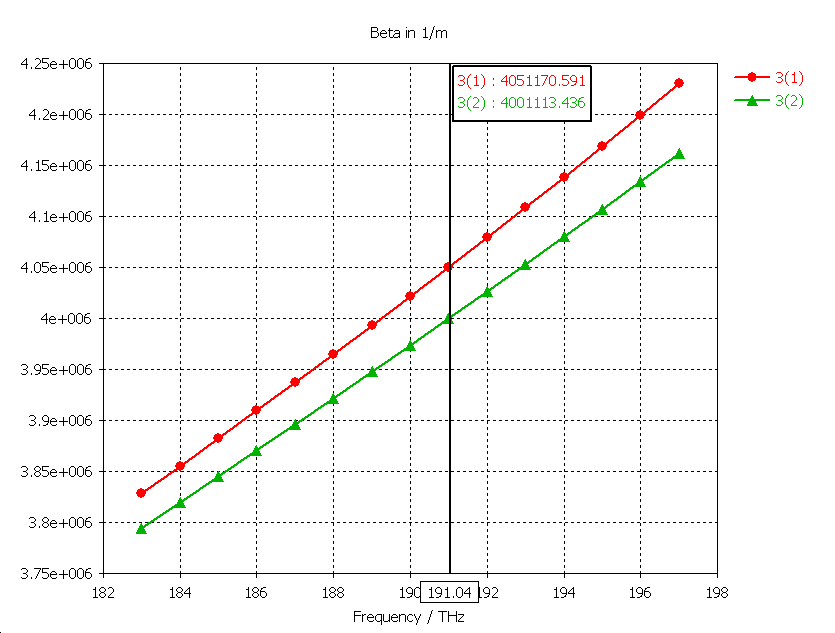
\includegraphics[width=0.9\textwidth]{4-effective-ri-200-230}
	\caption{Simulated effective propagation constant for the port modes in the cross-section of $\chem{Rib_{width}}$ = \SI{200}{\nano \meter}, $\chem{Rib_{height}}$ = \SI{110}{\nano \meter}, $\chem{Base_{width}}$ = \SI{230}{\nano \meter}, $\chem{Slab_{height}}$ = \SI{110}{\nano \meter}, obtained using CST simulation}
	\label{fig:4_effective_ri_200_230}
\end{figure}

\noindent The required length of the cross-section is obtained using \ref{eq:jones_matrix_wp1}. Since, $\beta_1$ = $4.051 \times 10^6$  and $\beta_2$ = $4.001 \times 10^6$. Hence, $L = \dfrac{\pi}{\beta_1 - \beta_2} \approx \SI{62}{\micro \meter}$. This means the length of the stair cross-section would be around \SI{62}{\micro \meter}. Effective \gls{ri} is dependent on frequency and so the cross-section length is also dependent on the frequency. The length is calculated at around $\SI{191}{\THz}$, so that the whole of the band ($\SI{184.48}{\THz}$ - $\SI{195.94}{\THz}$) can be covered for a relative good performance. This results could have also been obtained from COMSOL from the effective \gls{ri} calculation as shown in equation \ref{eq:lpi_calc}.

\begin{equation}\label{eq:lpi_calc}
L_\pi =  \dfrac {\pi} {\beta_1 - \beta_2} = \dfrac {\pi} {\dfrac {2\pi} {\lambda}\left(n_1 - n_2\right)} = \dfrac {\lambda} {2(n_1 - n_2)}
\end{equation}

\begin{figure}[H] %h
	\centering
	\includegraphics[width=0.9\textwidth]{4-wg-design-1}
	\caption{Design of single-stair waveguide with initial dimensions at the port as width = \SI{230}{\nano \meter} and height = \SI{220}{\nano \meter}. Stair cross-section dimensions are: $\chem{Rib_{width}}$ = \SI{200}{\nano \meter}, $\chem{Rib_{height}}$ = \SI{110}{\nano \meter}, $\chem{Base_{width}}$ = \SI{230}{\nano \meter}, $\chem{Slab_{height}}$ = \SI{110}{\nano \meter}, and cross-section length = \SI{62}{\micro\meter}. The output port is along the Z-axis, shown in the figure}
	\label{fig:4_wg_design_1}
\end{figure}

\noindent The 3D-design is simulated in CST with air cladding and with the previously estimated dimensions. The input and output ports are defined on the waveguide, which supports the two fundamental modes. As shown in Fig. \ref{fig:4_wg_design_1}, the stair cross-section can be envisaged if a Z-plane is cut in the asymmetric part of the waveguide.\\

\noindent Next, the S-parameters (transmission parameters) of the design are verified. The S-parameters are labelled as follows,
\begin{equation}\label{eq:s_parameter_label}
\mathrm{SA(M),B(N)},
\end{equation}
where A=output port, B=input port and M,N = mode number. For example, S2(2),1(1) means that input port is 1 and the mode is 1 whereas, output port is 2 and the mode at the output port is 2. Hence, S2(1),1(2) and S2(2),1(1) needs to be checked along with S2(1),1(1) and S2(2),1(2) for calculating the \gls{per}. The S-parameters obtained from the simulation shown in Fig. \ref{fig:4_stair_s_param_200_230} (for, 200$\times$\SI{230}{\nano \meter}) verifies that the model works according to the design principle with good \gls{per} over the C and L-band. 

%For example, the $PER_{191 THz} = 10 log_{10} $

\begin{figure}[H] %h
	\centering
	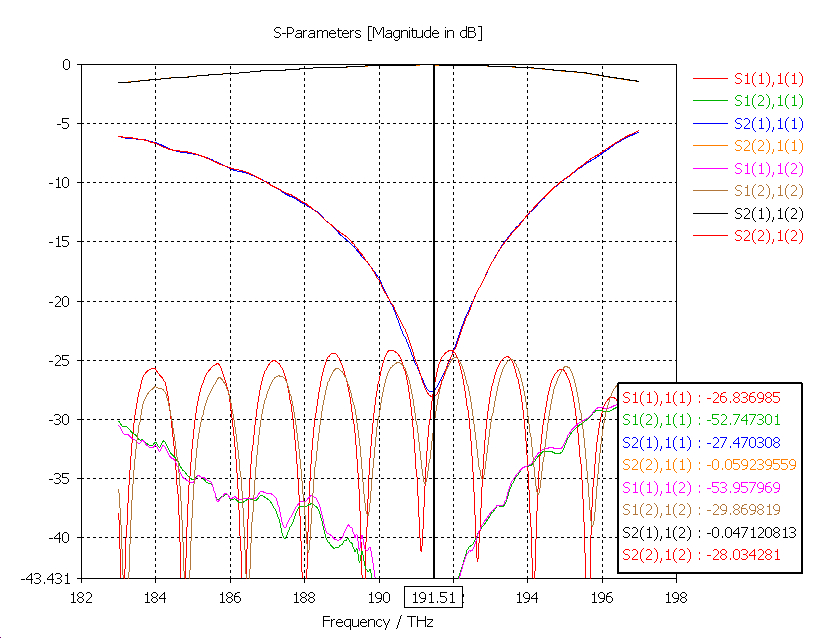
\includegraphics[width=0.9\textwidth]{4-stair-s-param-200-230}
	\caption{Simulated S-parameters in the single-stair waveguide with initial dimensions at the port as width = \SI{230}{\nano \meter} and height = \SI{220}{\nano \meter}. Stair cross-section dimensions are: $\chem{Rib_{width}}$ = \SI{200}{\nano \meter}, $\chem{Rib_{height}}$ = \SI{110}{\nano \meter}, $\chem{Base_{width}}$ = \SI{230}{\nano \meter}, $\chem{Slab_{height}}$ = \SI{110}{\nano \meter}, and cross-section length = \SI{62}{\micro\meter} obtained using CST 3-D simulation}
	\label{fig:4_stair_s_param_200_230}
\end{figure}

\begin{figure}[H] %h
	\centering
	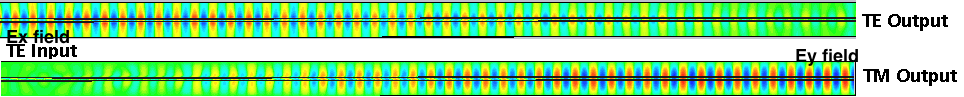
\includegraphics[width=\textwidth]{4-te-tm}
	\caption{TE-TM mode conversion along the waveguide with decreasing $\chem{E_{x}}$ field and increasing $\chem{E_{y}}$ field} 
	\label{fig:4_te_tm}
\end{figure}

\begin{figure}[H] %h
	\centering
	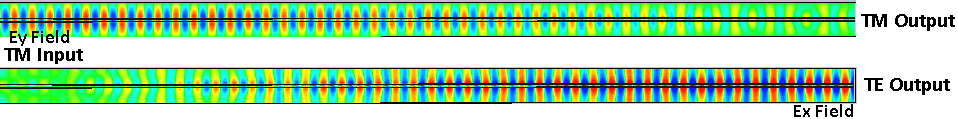
\includegraphics[width=\textwidth]{4-tm-te}
	\caption{TM-TE mode conversion along the waveguide with decreasing $\chem{E_{y}}$ field and increasing $\chem{E_{x}}$ field}
	\label{fig:4_tm_te}
\end{figure}

\subsubsection{Optimized dimensions of MEMS waveguide}
After finding the dimensions of the passive \gls{pr}, the \gls{mems} tunable waveguide was designed to cancel the effect of rotation. Intuitively, if any waveguide which is the mirror image of the bus waveguide is placed along side the bus waveguide, then \gls{pr} effect would be nullified. This is verified by plotting the graph in Fig. \ref{fig:4_graph_mode_sum_mems}. Since, at TE or TM mode, $E_X \gg E_Y$, or $E_Y \gg E_X$. Hence, $\left|\dfrac {Avg(E_{X_{mode}})} {Avg(E_{Y_{mode}})}\right| \rightarrow \infty$, or $\left|\dfrac {Avg(E_{Y_{mode}})} {Avg(E_{X_{mode}})}\right| \rightarrow \infty$, depending on \gls{te} or \gls{tm}-mode.
Hence, 
\begin{equation}\label{eq:mems_dim_eq}
\sum _{mode}Real\left| \log _{10}\dfrac {Avg(E_{X_{mode}})} {Avg(E_{Y_{mode}})}\right| \rightarrow \infty,
\end{equation}
and the maximum points on the graph will represent the dimensions of the \gls{mems} structure for which, there is no \gls{pr}. Logarithmic scale is used to plot the data in a manageable way. The supermodes are also verified in the cross-section in Fig. \ref{fig:4_mems_mode1_200_230} and Fig. \ref{fig:4_mems_mode2_200_230} to make sure higher order modes are not excited.

\begin{figure}[H] %h
	\centering
	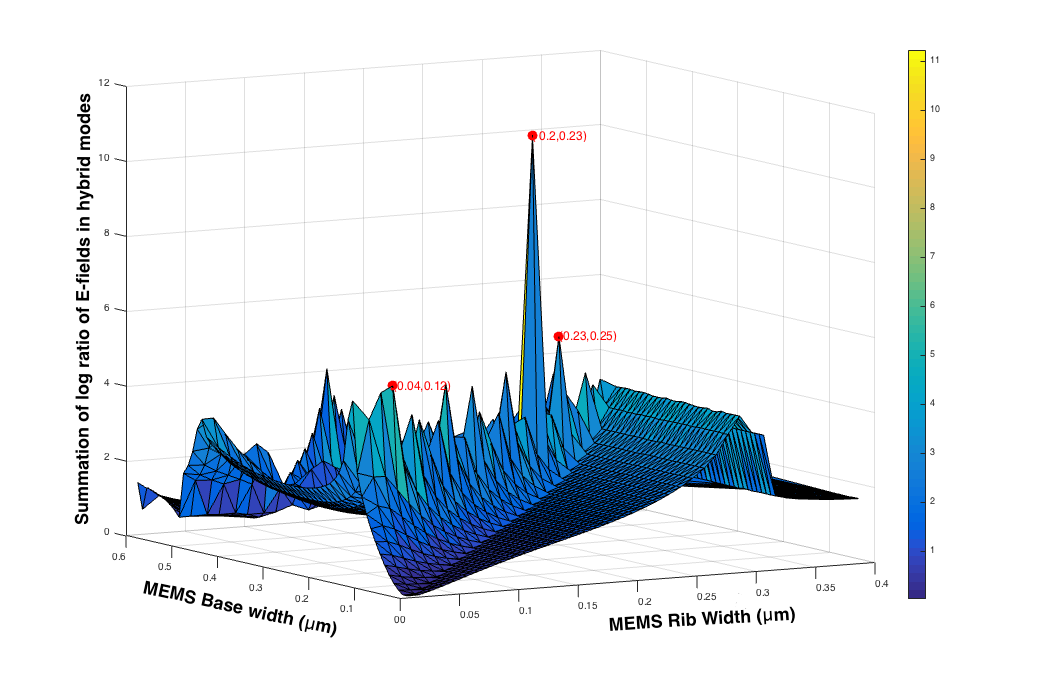
\includegraphics[width=1\textwidth]{4-graph-mode-sum-mems}
	\caption{Summation of real part of absolute value of the logarithmic ratio of $E_x$ and $E_y$ fields plotted against rib and total width in an area chart using MATLAB}
	\label{fig:4_graph_mode_sum_mems}
\end{figure}
		
\begin{figure}[H] %h
	\begin{subfigure}[t]{0.45\textwidth}
		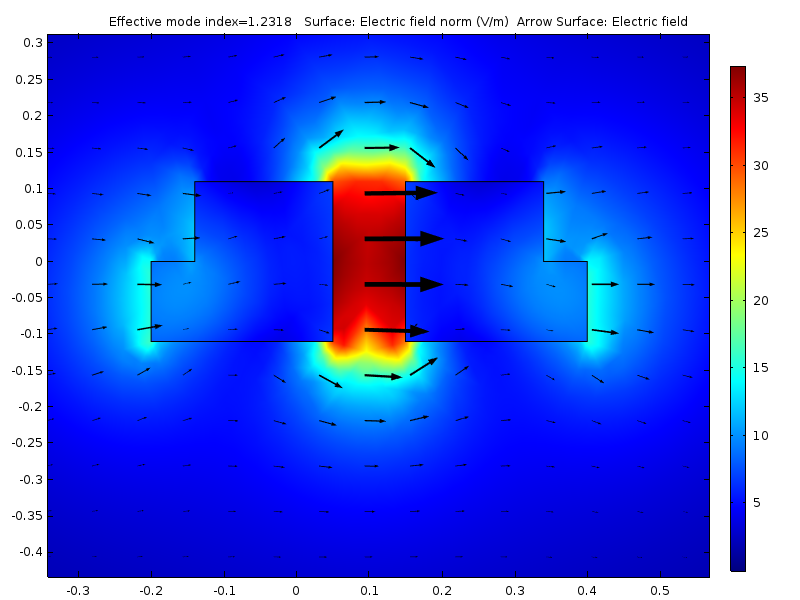
\includegraphics[width=\textwidth]{4-mems-mode1-200-230}
		\caption{\gls{te} mode with the \gls{mems} cross-section}
		\label{fig:4_mems_mode1_200_230}
	\end{subfigure}
	\hfill
	\begin{subfigure}[t]{0.45\textwidth}
		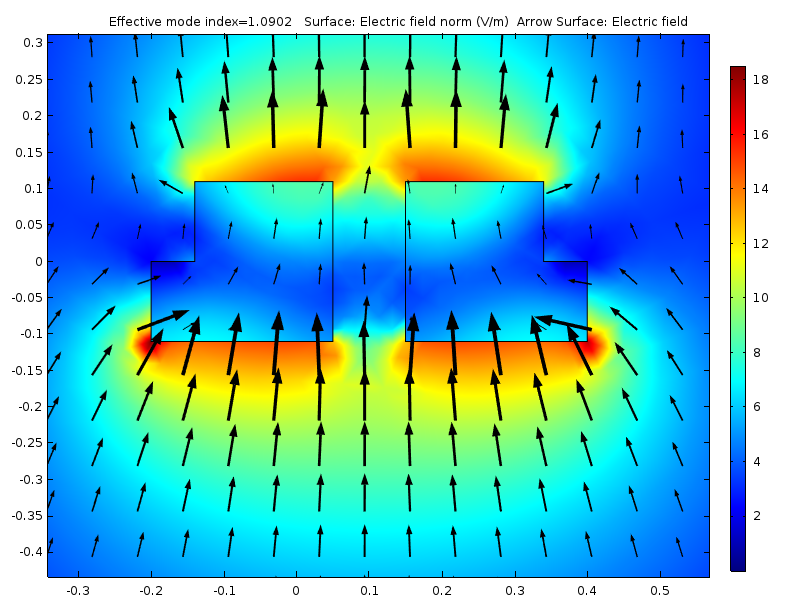
\includegraphics[width=\textwidth]{4-mems-mode2-200-230}
		\caption{\gls{tm} mode with the MEMS cross-section}
		\label{fig:4_mems_mode2_200_230}
	\end{subfigure}
	\caption{Modes in the cross-section with $\chem{Rib_{width}}$ = 200nm, $\chem{Slab_{width}}$ = \SI{30}{\nano \meter}, $\chem{Slab_{height}}$ = $\chem{Rib_{height}}$ = \SI{110}{\nano \meter}, in both bus and \gls{mems} waveguide, obtained using Comsol 2-D simulation}
\end{figure}

In this case the best dimensions for the \gls{mems} waveguide comes out as, $\chem{Rib_{width}}$ = \SI{200}{nano meter}, $\chem{Rib_{height}}$ = \SI{110}{nano meter}, $\chem{Base_{width}}$ = \SI{230}{nano meter}, $\chem{Slab_{height}}$ = \SI{110}{nano meter}. Fig. \ref{fig:4_mems_mode1_200_230} and Fig. \ref{fig:4_mems_mode2_200_230}, obtained using Comsol 2D simulation displays the port modes in the cross-section. This corroborates the claim that the \gls{mems} waveguide must be mirror image of the bus waveguide to inhibit \gls{pr}.

\subsubsection{Design of primary PR waveguide with MEMS waveguide}			
Based on the simulations performed and the dimensions of the cross-section obtained, the tunable \gls{pr} was designed as depicted in Fig. \ref{fig:4_wg_design_1_mems}. For quicker simulation the remaining portions of the cantilever in the \gls{mems} waveguide are not considered in the simulation design. Initially, a simulation was performed to check how the modes are guided in the slot with silica cladding as seen in Fig. \ref{fig:4_wg_tpr_mems_transmission}. However, for a \gls{mems} \gls{tpr} the waveguide has to be under-etched for free movement of the \gls{mems} cantilever to control polarization tuning. Hence, the cladding of a \gls{mems} \gls{tpr} is air. This scenario is simulated as shown in Fig. \ref{fig:4_wg_tpr_mems_transmission_air}. It can be observed that the \gls{mems} \gls{tpr} with air cladding is lossy due to reflection and scattering. 

\begin{figure}[H] %h
	\centering
	\includegraphics[width=0.5\textwidth]{4-wg-design-1-mems}
	\caption{Design of single-stair waveguide with MEMS tuning waveguide. Stair cross-section dimensions are: $\chem{Rib_{width}}$ = \SI{200}{\nano \meter}, $\chem{Rib_{height}}$ = \SI{110}{\nano \meter}, $\chem{Slab_{width}}$ = \SI{230}{\nano \meter}, $\chem{Slab_{height}}$ = \SI{110}{\nano \meter}, and Stair cross-section length = \SI{62}{\micro\meter}, in both the PR waveguide and MEMS waveguide. The output port is along the Z-axis}
	\label{fig:4_wg_design_1_mems}
\end{figure}

\begin{figure}[H] %h
	\centering
	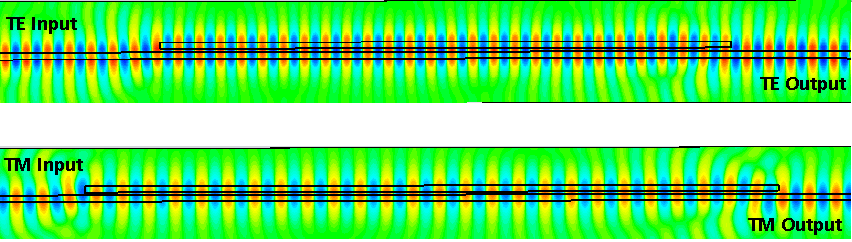
\includegraphics[width=1\textwidth]{4-wg-tpr-mems-transmission}
	\caption{\gls{tpr} transmission in silica cladding without \gls{mems} waveguide actuation}
	\label{fig:4_wg_tpr_mems_transmission}
\end{figure}

\begin{figure}[H] %h
	\centering
	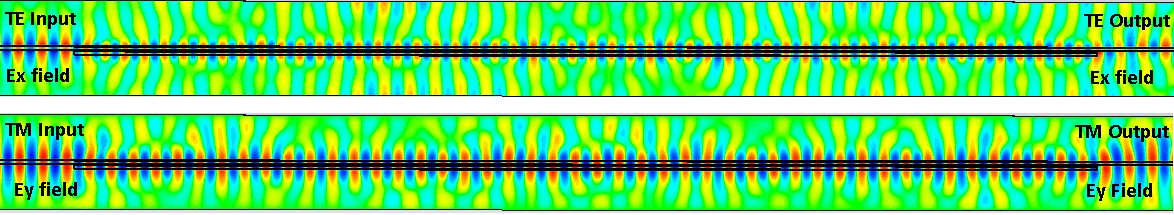
\includegraphics[width=1\textwidth]{4-wg-tpr-mems-transmission-air}
	\caption{\gls{tpr} transmission in air cladding without \gls{mems} waveguide actuation}
	\label{fig:4_wg_tpr_mems_transmission_air}
\end{figure}

\subsubsection{Device tolerance}
When fabricating devices in nanometer scale often it is very difficult to control the device dimensions precisely. Hence, a brief study on simulation level is performed to check for deviance resulting due to variations in etch depth during the fabrication process discussed later in section \ref{sec:fab_process}.\\  

Since the device layer thickness used in the fabrication process is of height \SI{220}{\nano \meter}, the different etch depths considered are \SI{100}{\nano \meter} and \SI{130}{\nano \meter} which corresponds to \SI{120}{\nano \meter} and \SI{90}{\nano \meter} slab height respectively. Fist 20 minimum values of $\sum _{mode}Real\left| \log _{10}\dfrac {E_{X_{mode}}} {E_{Y_{mode}}}\right|$, is plotted against $\chem{Rib_{width}}$ and $\chem{Slab_{width}}$ in the following figure in Fig. \ref{fig:4_graph_mode_sum_120nm_slab_height} for an etch depth of 100nm. 

\begin{figure}[H] %h
	\centering
	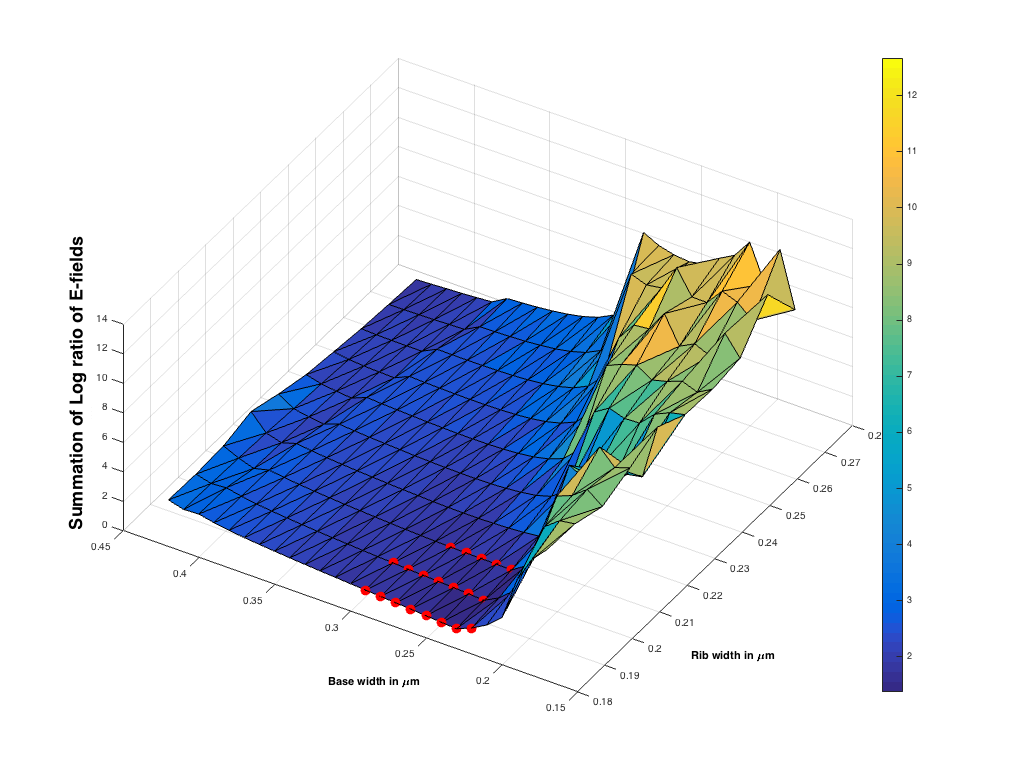
\includegraphics[width=1\textwidth]{4-graph-mode-sum-120nm-slab-height}
	\caption{20 least values, representing the summation of real part of absolute value of the logarithmic ratio of $E_x$ and $E_y$ fields, plotted against rib and total width in an area chart using MATLAB for $\chem{Slab_{height}}$ = \SI{120}{\nano \meter}}
	\label{fig:4_graph_mode_sum_120nm_slab_height}
\end{figure}
\noindent It can be seen in the above Fig. \ref{fig:4_graph_mode_sum_120nm_slab_height} that the hybridized modes appear to be at $45^{\circ}$ around $\chem{\SI{230}{\nano \meter} \leq Base_{width} \leq \SI{300}{\nano \meter}}$ and $\chem{\SI{170}{\nano \meter} \leq Rib_{width} \leq \SI{200}{\nano \meter}}$. So, if the $\chem{Rib_{width}}$ and $\chem{Base_{width}}$ are controlled in the fabrication process, the device can still function and needs to be characterized accordingly.\\

The same process is followed for a speculated etch depth of \SI{130}{\nano \meter} and the 20 best dimensions are plotted which comes out to be $\chem{\SI{240}{\nano \meter} \leq Base_{width} \leq \SI{300}{\nano \meter}}$ and $\chem{\SI{160}{\nano \meter} \leq Rib_{width} \leq \SI{200}{\nano \meter}}$. The exact pairs can be identified in the Fig. \ref{fig:4_graph_mode_sum_90nm_slab_height}.
\begin{figure}[H] %h
	\centering
	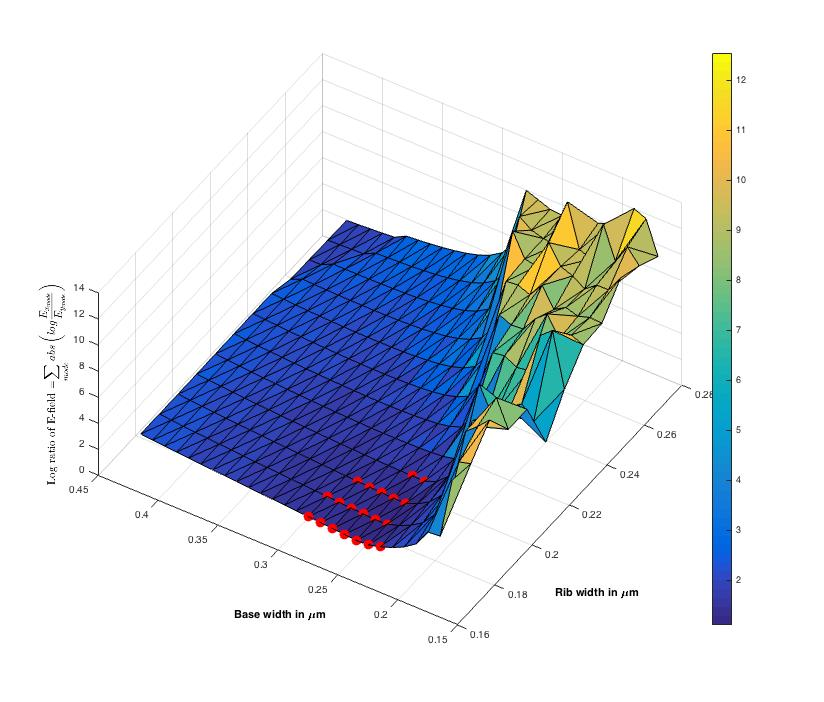
\includegraphics[width=1\textwidth]{4-graph-mode-sum-90nm-slab-height}
	\caption{20 least values, representing the summation of real part of absolute value of the logarithmic ratio of $\chem{E_x}$ and $\chem{E_y}$ fields, plotted against rib and total width in an area chart using MATLAB for Slab height = \SI{90}{\nano \meter}}
	\label{fig:4_graph_mode_sum_90nm_slab_height}
\end{figure}

\begin {table}[H]
\begin{center} 
	\begin{tabular}{ | m{6em} | m{6em}| m{6em} | m{6em} | }  
		\hline
		\textbf{Etch depth (nm)} & \textbf{Slab height (nm)} & \textbf{Base width (nm)} & \textbf{Rib width (nm)} \\
		\hline\hline
		100 & 120 & 230 & 180 \\
		\hline
		100 & 120 & 240 & 180 \\ 
		\hline
		100 & 120 & 250 & 180 \\ 
		\hline
		100 & 120 & 260 & 180 \\ 
		\hline
		100 & 120 & 270 & 180 \\ 
		\hline
		100 & 120 & 280 & 180 \\ 
		\hline
		100 & 120 & 290 & 180 \\ 
		\hline
		100 & 120 & 300 & 180 \\ 
		\hline
		100 & 120 & 240 & 190 \\ 
		\hline
		100 & 120 & 250 & 190 \\ 
		\hline
		100 & 120 & 260 & 190 \\ 
		\hline
		100 & 120 & 270 & 190 \\ 
		\hline
		100 & 120 & 280 & 190 \\ 
		\hline
		100 & 120 & 290 & 190 \\ 
		\hline
		100 & 120 & 300 & 190 \\ 
		\hline	
		100 & 120 & 240 & 200 \\ 
		\hline
		100 & 120 & 250 & 200 \\ 
		\hline
		100 & 120 & 260 & 200 \\ 
		\hline	
		100 & 120 & 270 & 200 \\ 
		\hline
		100 & 120 & 280 & 200 \\ 
		\hline
		130 & 90 & 240 & 170 \\ 
		\hline
		130 & 90 & 250 & 170 \\ 
		\hline
		130 & 90 & 260 & 170 \\ 
		\hline
		130 & 90 & 270 & 170 \\ 
		\hline
		130 & 90 & 280 & 170 \\ 
		\hline
		130 & 90 & 290 & 170 \\ 
		\hline
		130 & 90 & 300 & 170 \\ 
		\hline
		130 & 90 & 250 & 180 \\ 
		\hline
		130 & 90 & 260 & 180 \\ 
		\hline
		130 & 90 & 270 & 180 \\ 
		\hline
		130 & 90 & 280 & 180 \\ 
		\hline
		130 & 90 & 290 & 180 \\ 
		\hline
		130 & 90 & 300 & 180 \\ 
		\hline
		130 & 90 & 250 & 190 \\ 
		\hline
		130 & 90 & 260 & 190 \\ 
		\hline
		130 & 90 & 270 & 190 \\ 
		\hline
		130 & 90 & 280 & 190 \\ 
		\hline
		130 & 90 & 290 & 190 \\ 
		\hline
		130 & 90 & 250 & 200 \\ 
		\hline
		130 & 90 & 260 & 200 \\ 
		\hline
	\end{tabular}
\end{center}
\caption {Device dimensions for obtaining the hybridized modes at different etch-depths} \label{table:device_tolerance} 
\end {table}

\begin{comment}

		\subsection{Design B: Tapered Si waveguide with horizontal gradual asymmetry on SOI with air cladding based on mode evolution}

\subsubsection{Optimized dimensions of bus waveguide}
		
\begin{figure}[H] %h
	\begin{subfigure}[t]{0.45\textwidth}
		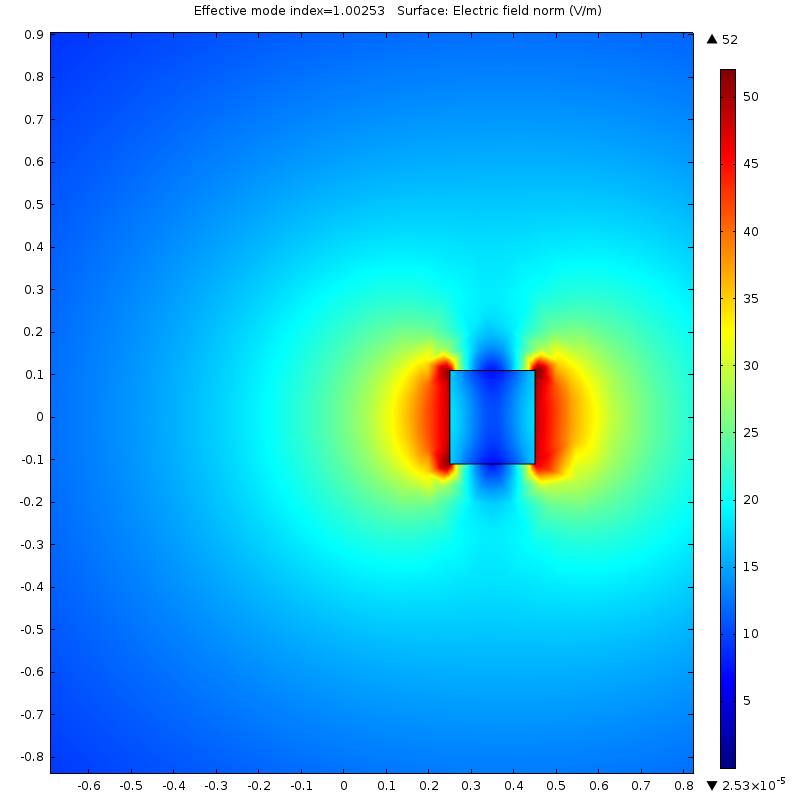
\includegraphics[width=\textwidth]{3-mode1-200-200}
		\caption{\gls{te} mode in the cross-section}
		\label{fig:4_mode1_200_200}
	\end{subfigure}
	\hfill
	\begin{subfigure}[t]{0.45\textwidth}
		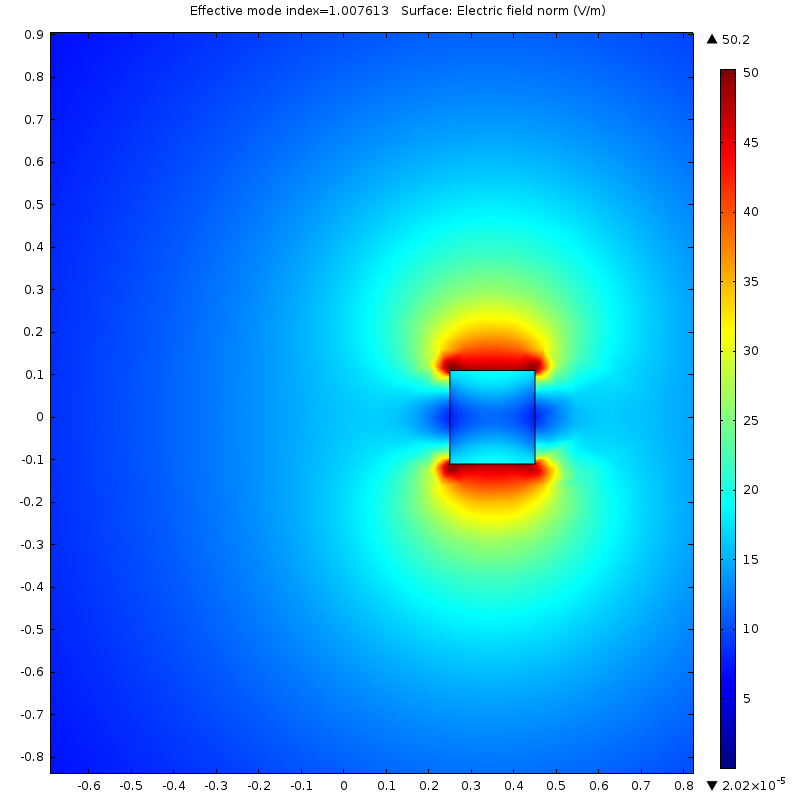
\includegraphics[width=\textwidth]{3-mode2-200-200}
		\caption{\gls{tm} mode in the cross-section}
		\label{fig:4_mode2_200_200}
	\end{subfigure}
	\caption{Hybrid modes in the cross-section with width = 200nm, height = 220nm, obtained using Comsol 2-D simulation}
\end{figure}

\subsubsection{Optimized dimensions of MEMS waveguide}	

\subsubsection{Device tolerance}

\subsubsection{Representational design based on simulation}
\end{comment}

\section{Designing auxiliary components for measurement setup}
To test the \gls{tpr} auxiliary components like grating couplers (\gls{te} \& \gls{tm}), tapers, \gls{pbs} are designed. The gratings are designed in way to couple \gls{te} and \gls{tm}-modes from the LASER to the waveguide. However the gratings have a width of \SI{12}{\micro \meter} whereas, the \gls{tpr} section in the waveguide has width of \SI{230}{\nano \meter}. Hence, tapers are used to reduce the mode size and guide light into the \gls{tpr} section. Finally, a \gls{pbs} is designed which again splits the \gls{te} and \gls{tm}-modes and guides them to the \gls{te} and \gls{tm} grating couplers respectively via tapers where a photo-detector measures the intensity of output light. Another approach like butt-coupling can be used. But it is difficult to couple light into narrow waveguides in a low-loss manner as the mode size in fiber core is bigger than the mode size in the waveguide.  

\begin{figure}[H] %h
	\centering
	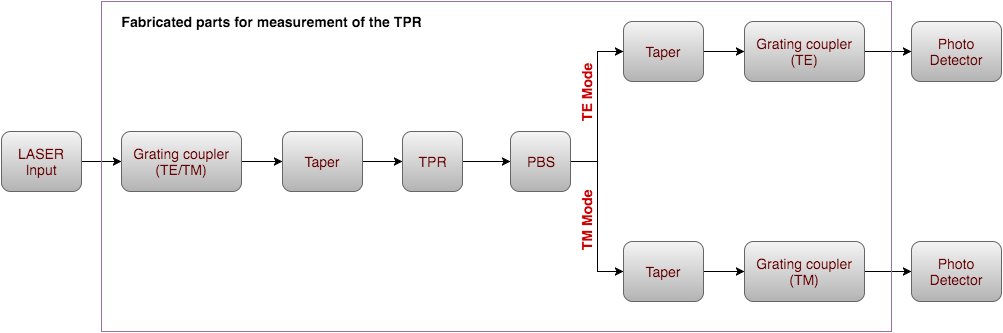
\includegraphics[width=1\textwidth]{4-sys-design}
	\caption{System level block diagram of the fabricated measurement setup}
	\label{fig:4_sys_design}
\end{figure}
\noindent In the Fig. \ref{fig:4_sys_design} a high level block diagram of the measurement setup is shown. Whereas, in Fig. \ref{fig:4_tpr_test_setup} schematic top view of the actual system design is shown with gratings, tapers, \gls{tpr}, \gls{tm} coupler and bridges. 
\begin{figure}[H] %h
	\centering
	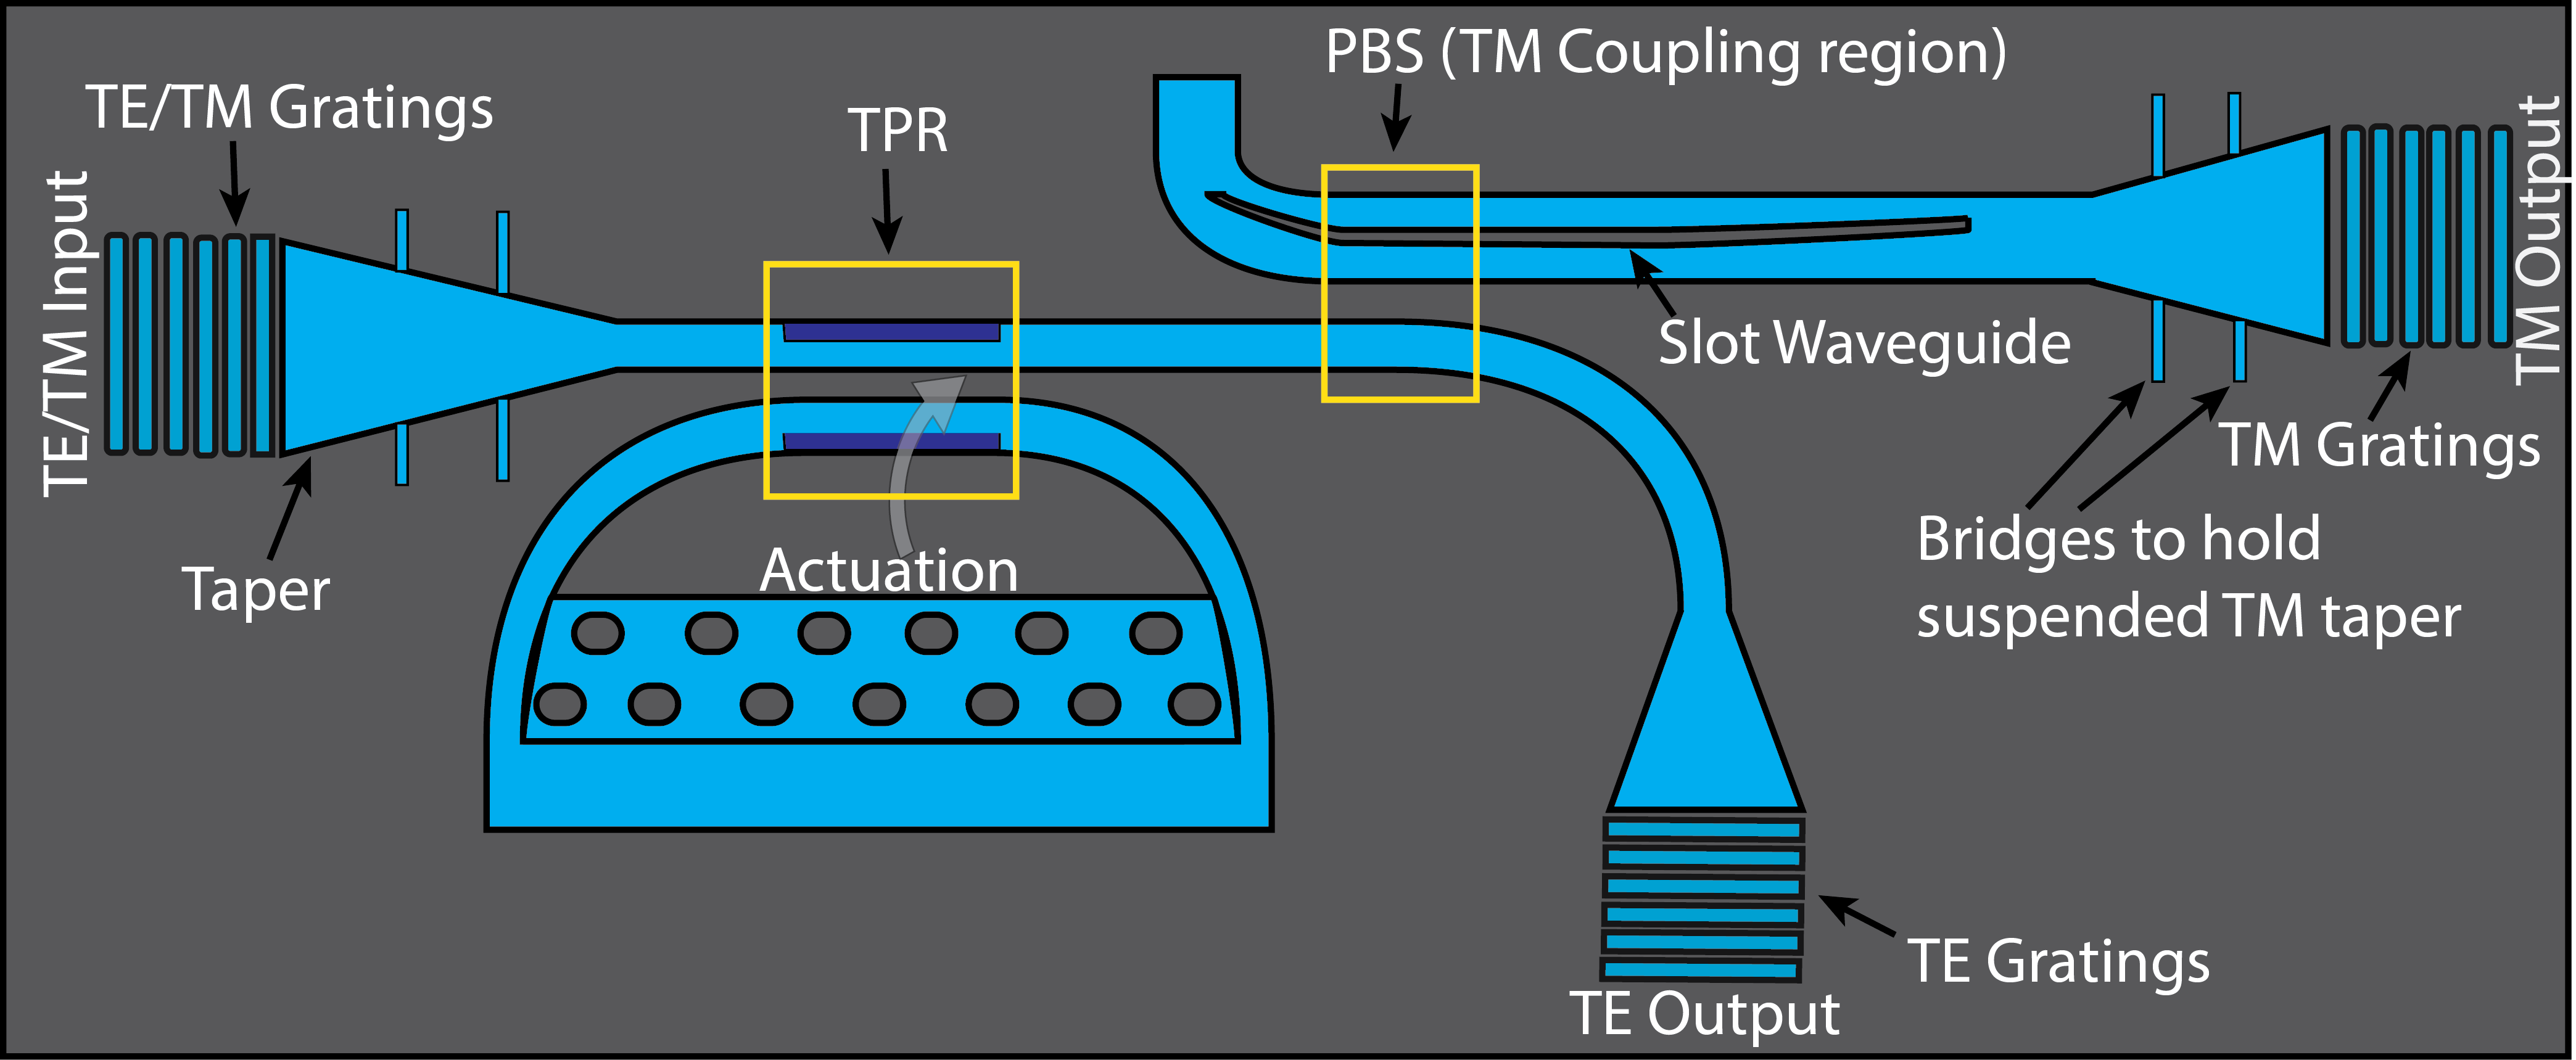
\includegraphics[width=1\textwidth]{4-tpr-test-setup}
	\caption{Low level schematic representation of the fabricated measurement setup}
	\label{fig:4_tpr_test_setup}
\end{figure}

\subsection{Grating coupler design}
The high effective index and small mode dimensions of single mode silicon waveguides makes fiber coupling challenging. Waveguide-to-fiber surface grating couplers with fill factor apodization offer low back reflection into the silicon waveguide and a single required lithography step. Using surface grating couplers, the mode matching problem can be solved by expanding the width of the on-chip silicon waveguide, and etching a grating into the expanded section that diffracts light out of plane into a fiber, placed at certain angle to the normal. The approach taken increases the coupling efficiency by tailoring the leakage factor of the grating to the mode profile of the fiber. The main benefits of this approach are a low back reflection into the silicon waveguide and high efficiency in the coupling \cite{grating_coupler}. In the design, the gratings used are \SI{12}{\micro\meter} wide which narrows down to a width of \SI{230}{\nano\meter} in the \gls{pr} section. The approach is shown in Fig. \ref{fig:4_gc_setup}. Also, two types of gratings are designed for \gls{te} and \gls{tm} coupling. The \gls{tm} gratings are under-etched to avoid coupling of the deconfined \gls{tm} modes in the $\chem{SiO_{2}}$. Whereas, since \gls{te} modes are confined, the gratings are not under-etched. 

\begin{figure}[H] %h
	\begin{subfigure}[t]{0.45\textwidth}
		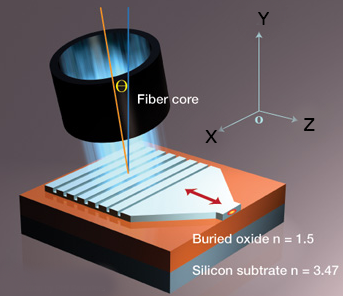
\includegraphics[width=\textwidth]{4-gc-setup}
		\caption{Fiber to waveguide surface coupling using grating coupler}
		\label{fig:4_gc_setup}
	\end{subfigure}
	\hfill
	\begin{subfigure}[t]{0.45\textwidth}
		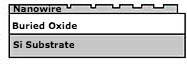
\includegraphics[width=\textwidth]{4-gc-cross-section}
		\caption{Apodized grating coupler cross-section}
		\label{fig:4_gc_cross_section}
	\end{subfigure}
	\caption{Overview of surface coupling from fiber to waveguide using apodized grating coupler with cross-sectional view}
\end{figure}


\subsection{Taper with bridge design}
While tapering down to the \gls{tpr} cross-section from the grating coupler cross-section, the $\chem{SiO_{2}}$ underneath is etched away for \gls{tm} input. Hence, to support the structure from the side bridges are constructed which forms a slab like structure at certain cross-sections. These kinds of structures accommodate mode conversions between $\chem{TM_0}$ and $\chem{TE_3}$. Also, these bridges are constructed in other places in the waveguide structure where support is necessary to hold the waveguide. For example, if the core waveguide width is \SI{700}{\nano\meter} then a total base width (core and bridge) of \SI{1500}{\nano\meter} must be avoided for mode conversion reasons, as simulated and plotted using COMSOL in Fig. \ref{fig:4_slab_modes_700nm}. As, it can be seen that around \SI{1500}{\nano\meter} base width there is a mode conversion between $\chem{TM_0}$ and $\chem{TE_3}$ represented in Fig. \ref{fig:4_te_1500_slab} and Fig. \ref{fig:4_tm_1500_slab}. However, there is no mode conversion between $\chem{TM_0}$ and $\chem{TE_2}$, since the field distributions are not similar and hence they do not couple.
 
 \begin{figure}[H] %h
 	\centering
 	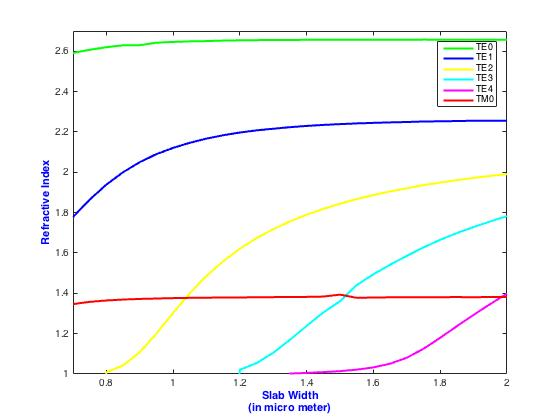
\includegraphics[width=.75\textwidth]{4-slab-modes-700nm}
 	\caption{TE and TM modes at different base widths obtained using COMSOL mode solvers}
 	\label{fig:4_slab_modes_700nm}
 \end{figure}
 
 \begin{figure}[H] %h
 	\begin{subfigure}[t]{0.45\textwidth}
 		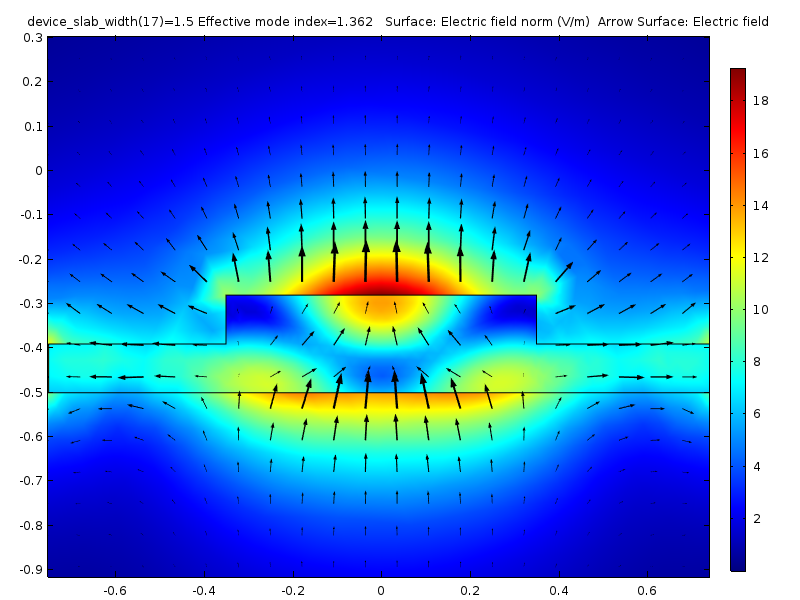
\includegraphics[width=\textwidth]{4-te-1500-slab}
 		\caption{TE mode with $\chem{Base_{width}}$ = \SI{1500}{\nano\meter}}
 		\label{fig:4_te_1500_slab}
 	\end{subfigure}
 	\hfill
 	\begin{subfigure}[t]{0.45\textwidth}
 		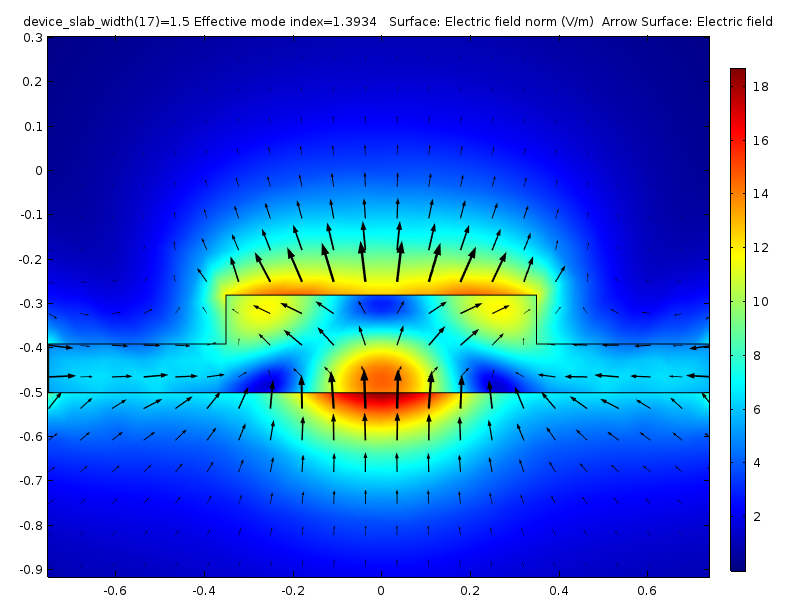
\includegraphics[width=\textwidth]{4-tm-1500-slab}
 		\caption{TM mode with $\chem{Base_{width}}$ = \SI{1500}{\nano\meter}}
 		\label{fig:4_tm_1500_slab}
 	\end{subfigure}
 	\caption{Mode conversion in Slab modes at $\chem{Base_{width}}$ = \SI{1500}{\nano\meter}, obtained using Comsol 2-D simulation having same effective index}
 \end{figure}


\subsection{Polarization beam splitter design}
The \gls{pbs} is based on an asymmetric directional coupler utilizing the evanescent coupling between a strip-waveguide and a nanoslot waveguide \cite{pbs_dai_2011}. First, effective \gls{ri} is calculated for different core widths with height = \SI{220}{\nano \meter}. The results are displayed in Fig. \ref{fig:4_pbs_core_waveguide}.
\begin{figure}[H] %h
	\centering
	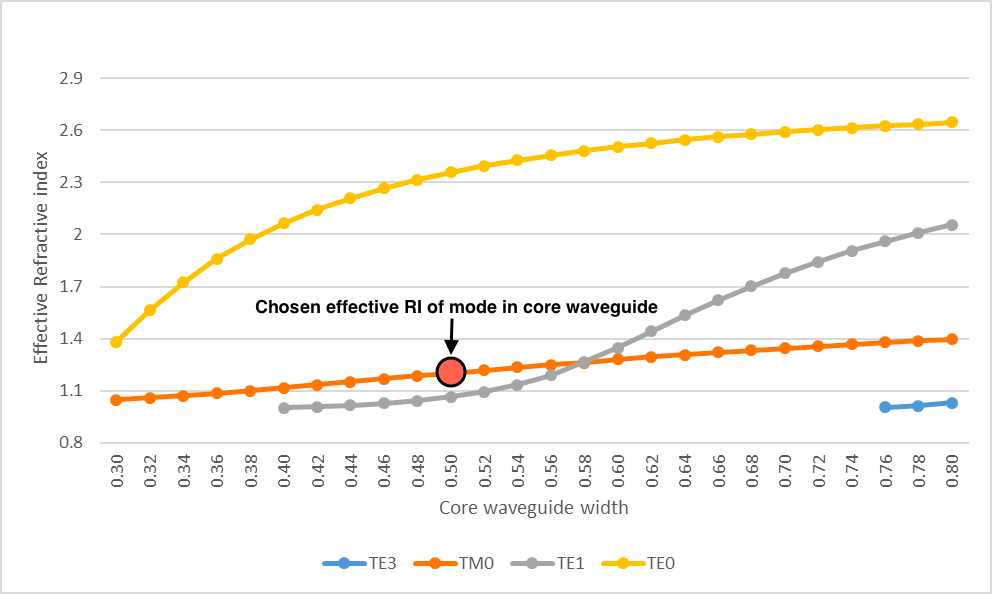
\includegraphics[width=0.75\textwidth]{4-pbs-core_waveguide}
	\caption{Effective \gls{ri} for different dimensions of core waveguide width}
	\label{fig:4_pbs_core_waveguide}
\end{figure}
\noindent Next, the effective \gls{ri} is calculated for the four lowest order modes at different widths of nanoslot waveguide with a height of \SI{220}{\nano \meter} and slot width of \SI{100}{\nano \meter}. The gap between the strip-nanowire and the nanoslot waveguide is \SI{150}{\nano \meter}. The results are plotted in Fig. \ref{fig:4_pbs_slot_waveguide}.
\begin{figure}[H] %h
	\centering
	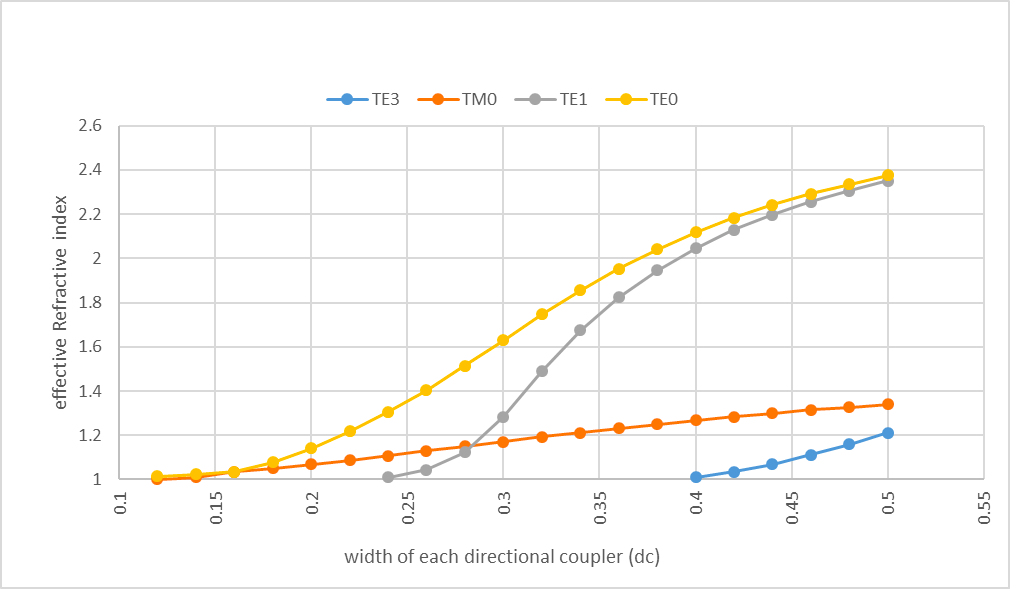
\includegraphics[width=0.75\textwidth]{4-pbs-slot_waveguide}
	\caption{Effective \gls{ri} for different dimensions of slot cross-section}
	\label{fig:4_pbs_slot_waveguide}
\end{figure}
\noindent It can be seen in Fig. \ref{fig:4_pbs_core_waveguide} that the effective index of $\chem{TM_0}$ at a width of \SI{500}{\nano \meter} is 1.20. Whereas, it can be seen in Fig. \ref{fig:4_pbs_slot_waveguide} that the effective index of 1.20 in $\chem{TM_0}$ is obtained around a width of \SI{330}{\nano \meter} for each section of the nanoslot waveguide. Also, the supermodes are checked in the cross-section of the nanoslot waveguide (with a nano-strip in the coupling waveguide) to understand the coupled modes shown in Fig. \ref{fig:4_pbs_te_coupling}, Fig. \ref{fig:4_pbs_tm_coupling} and Fig. \ref{fig:4-pbs-tm-anti-coupling}.
\begin{figure}[H] %h
	\centering
	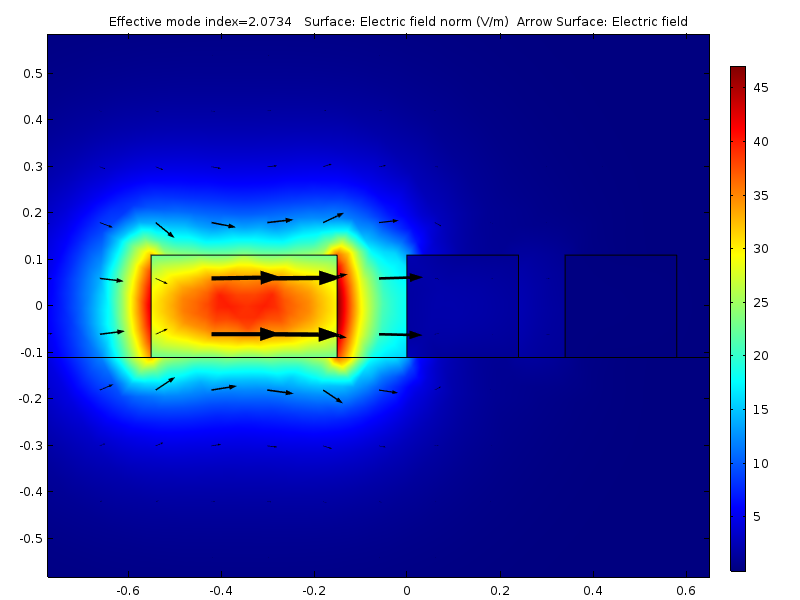
\includegraphics[width=0.45\textwidth]{4-pbs-te-coupling}
	\caption{No \gls{te} coupling in \gls{pbs} slot waveguide at the mode coupling region}
	\label{fig:4_pbs_te_coupling}
\end{figure}

\begin{figure}[H] %h	
	\begin{subfigure}[t]{0.45\textwidth}
		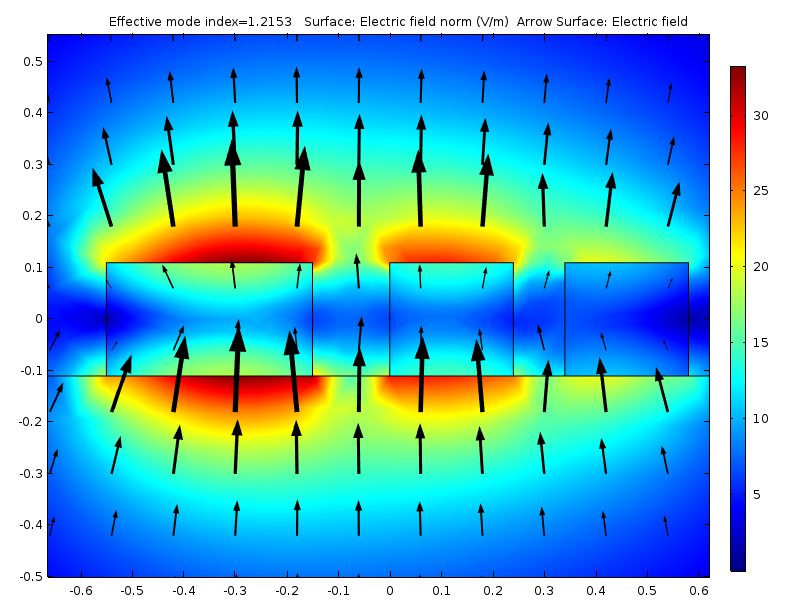
\includegraphics[width=\textwidth]{4-pbs-tm-coupling}
		\caption{Phase matched \gls{tm} coupling in the mode coupling cross-section}
		\label{fig:4_pbs_tm_coupling}
	\end{subfigure}
	\hfill
	\begin{subfigure}[t]{0.45\textwidth}
		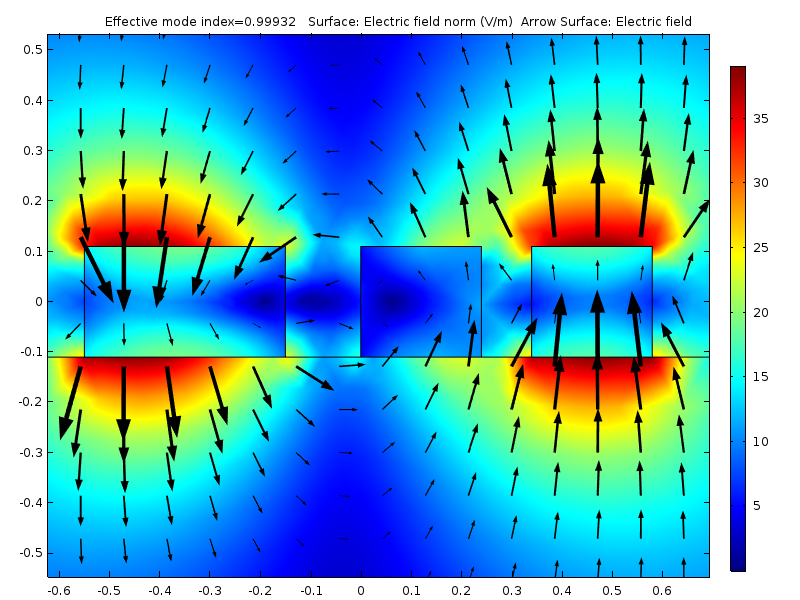
\includegraphics[width=\textwidth]{4-pbs-tm-anti-coupling}
		\caption{Phase mismatched \gls{tm} coupling in the mode coupling cross-section}
		\label{fig:4-pbs-tm-anti-coupling}
	\end{subfigure}	
	\caption{\gls{tm} coupling in \gls{pbs} slot waveguide at the mode coupling region for different phases}
\end{figure}

\noindent Finally, the design is simulated in 3-D using CST for checking the transmission with strip-nanowire of width \SI{500}{\nano \meter} and nanoslot waveguide of width \SI{330}{\nano \meter} each with slot width of \SI{100}{\nano \meter}. The coupling length is estimated from equation \ref{eq:lpi_calc}. As, $\chem{n_{TM}}$ (Phase matched) $\approx$ 1.20 and $\chem{n_{TM}}$ (Phase mismatched) $\approx$ 1.00, hence, at \SI{1550}{\nano \meter},

\begin{equation}\label{eq:lpi_calc_mc}
\mathrm{L_\pi} = \dfrac {\lambda} {2(n_1 - n_2)} = \dfrac {1550} {2\times(1.2 - 1.00)} = \SI{3.875}{\micro \meter}.
\end{equation} 

\noindent As seen in Fig. \ref{fig:4_te_coupler}, the \gls{te} mode goes through without coupling. Whereas, as seen in Fig. \ref{fig:4_tm_coupler}, the \gls{tm} mode crosses through efficiently in the coupling region. As, it can be seen some portion of the \gls{tm} mode goes through as well. However, the measured \gls{per} is more than \SI{20}{\decibel} in the simulation. The purpose of this setup is to make sure that both \gls{te} and \gls{tm} modes can be measured at different ports. In the final design of the measurement setup the nanoslot waveguide is not bent after the coupling region to minimize losses for \gls{tm} mode. As \gls{tm} mode is highly deconfined, bends can cause lossy transmission for \gls{tm} modes. Whereas, since \gls{te} mode is confined, the strip-nanowire core waveguide is given a sharp bend to minimize coupling beyond the coupling region. The idea can be viewed in Fig. \ref{fig:4_tpr_test_setup}.

\begin{figure}[H] %h
	\begin{subfigure}[t]{0.45\textwidth}
		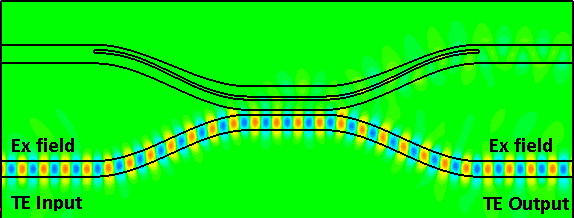
\includegraphics[width=\textwidth]{4-te-coupler}
		\caption{\gls{te} mode through}
		\label{fig:4_te_coupler}
	\end{subfigure}
	\hfill
	\begin{subfigure}[t]{0.45\textwidth}
		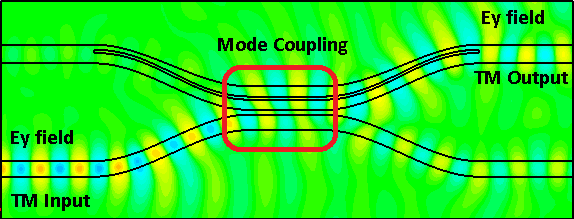
\includegraphics[width=\textwidth]{4-tm-coupler}
		\caption{\gls{tm} mode crossing at the coupling region}
		\label{fig:4_tm_coupler}
	\end{subfigure}
	\caption{\gls{te} and \gls{tm} mode propagation in a waveguide with \gls{pbs} section. \gls{te} mode goes through, whereas, the \gls{tm} mode crosses at the \gls{pbs} region due to mode matching of the two waveguides in the \gls{pbs} section}
\end{figure}


\end{document}
